\subsection{Empirical Testbed Experiment}
In the empirical testbed measurement experiment, we positioned a pair of testbed nodes in an increasing distance from each other, on an outdoor olympic running track, starting from 0 meters (the nodes were located on top of each other) up to 120 meters, in an open field with minimal obstacles to signal propagation.
At first, one node was powered on and fixed static to a location, and set as the advertiser node. The other node was placed in an appropriate distance, and a Python script was used to scan for BLE advertisements from the first node. The RSSI value, transmitting power, and the timestamp at time of reception were logged for each advertisement received. For every such configuration the logging node scanned for two minutes, paused for a short while to let the antenna cool down, and repeated the scanning for twenty times.
As an advertising node, the tool $bluetoothctl$ was used to register BLE advertisements, which advertised the node name, transmitting power, and most importantly set the advertisement interval.
Due to technical hardware reasons, we are not able to control the transmission power of the BLE advertisements, and it was recorded to be the same across all measurements: 12 dBm. The wireless chip Cypress CYW43455, as supported by our testbed nodes Raspberry Pi 3B+, does not let us change the used transmission power; a point for future research could be to measure the maximum achieved distance with varying transmitting power levels using a different chip or a wireless dongle.
Furthermore, we were not able to have fine-grain control over exactly when the advertisements were sent, because the BlueZ Bluetooth communication stack and the underlying hardware controller handle the advertisement scheduling internally to prevent antenna overheating.
To best mitigate this, we set the advertisement interval window to the minimum possible values of [20 ms, 20 ms] to achieve the highest consistent frequency of advertisements sent. We were however able to prove that the advertisements were not actually being consistently sent with the configured interval window of 20ms using a Bluetooth sniffer on a mobile phone, which measured the actual advertisement intervals: these fluctuated around 20-100ms.
Another point for future research would be to develop a Bluetooth driver that allows fine-grain control over the advertising scheduling: for that the \texttt{python-dbus} library could be used to directly interface with the underlying communication data bus, D-Bus.

\subsection{Results}
 \begin{figure}[htbp]
     \centering
     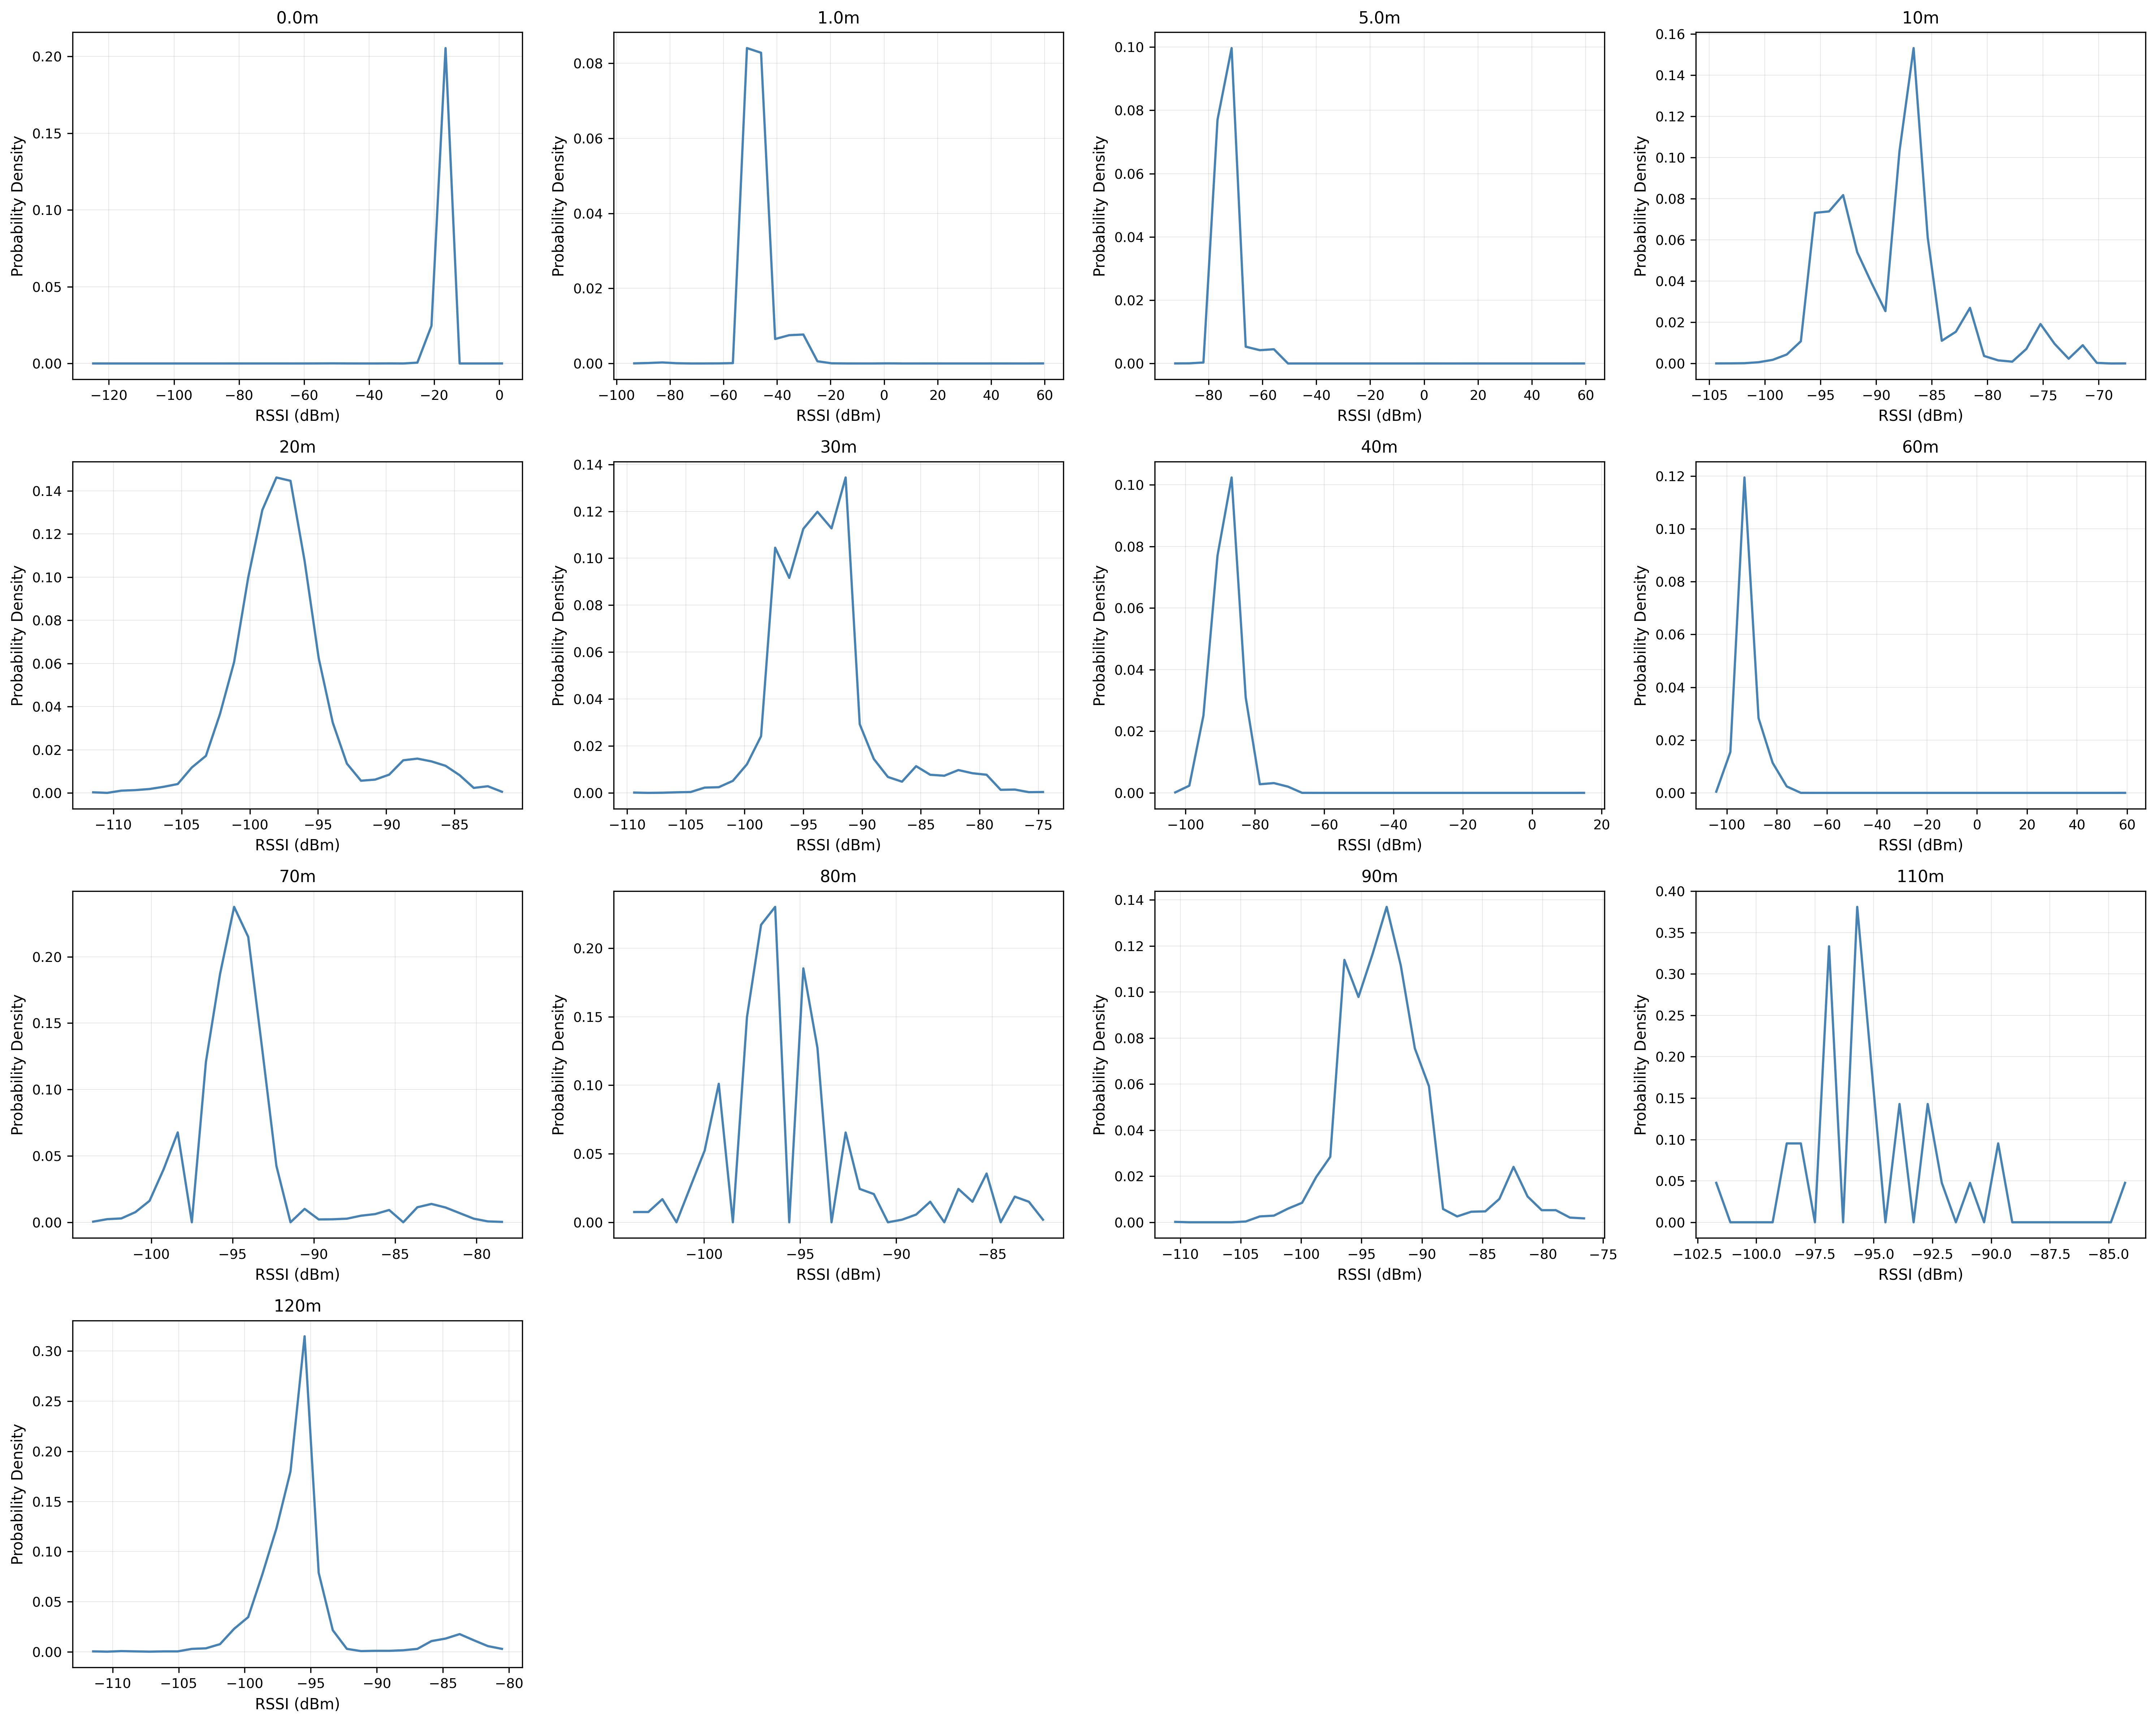
\includegraphics[width=0.5\textwidth]{figures/rssi_density_subplots.png}
     \caption{RSSI KDE plot at different distances}
     \label{fig:rssi-density}
 \end{figure}
Figure \ref{fig:rssi-density} shows the Kernel Density Estimation (KDE) plots of the RSSI values recorded at different distances, using 30 bins for the RSSI values. We can see that most distances exhibit a normal distribution of values where most values are centered around the mean, with some outliers, while some distances exhibit a jittery behavior, attributed to passing temporary environmental interference.
Generally, it is easy to see a correlation between an increase in the distance and a decrease in the RSSI value.

\begin{figure}[htbp]
     \centering
     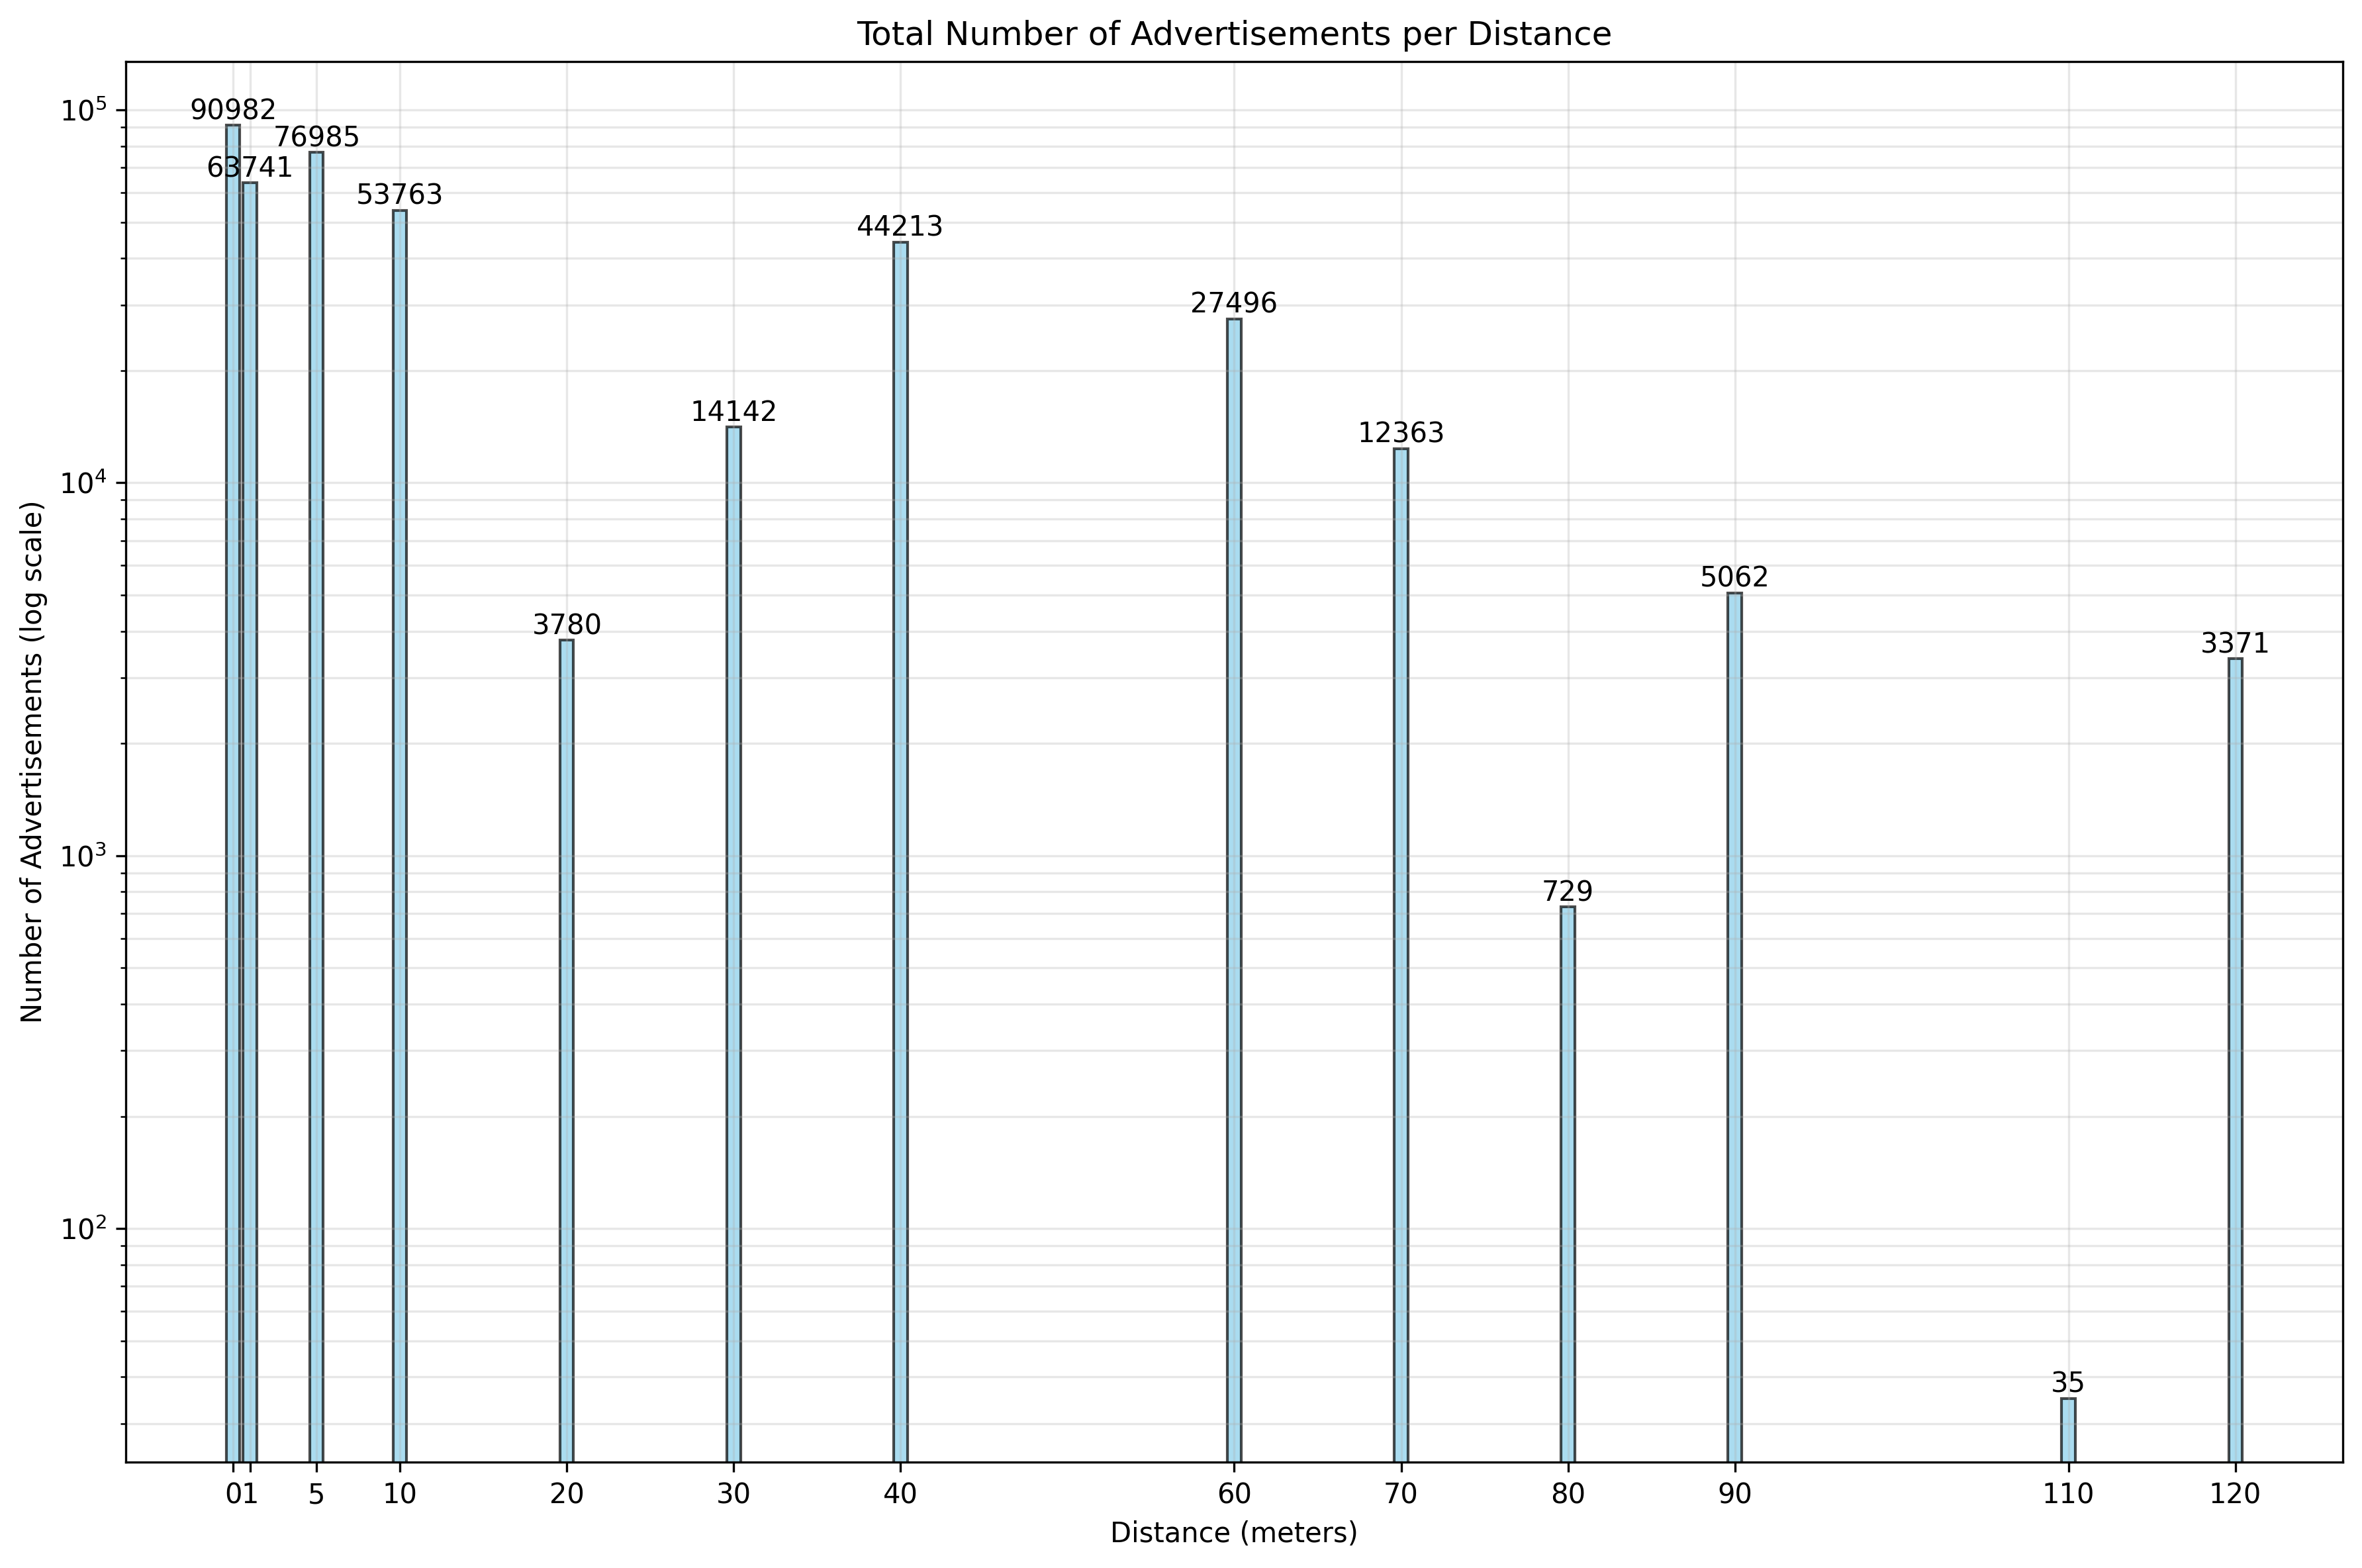
\includegraphics[width=0.5\textwidth]{figures/advertisements_per_distance.png}
     \caption{Number of advertisements received at different distances}
     \label{fig:advertisements-distance}
 \end{figure}

Figure \ref{fig:advertisements-distance} shows the number of advertisements received at different distances. There is strong negative trend between the distance and the number of advertisements received, as expected.
We can also here observe a sudden unexpected drop in the number of advertisements received (for example, at 20 meters), which we again attribute to temporary environmental interference (e.g. runners at the track passing by the experiment obstructing the clear path, sometimes with phones or other metal objects in their pockets that reflect the signals and cause more wireless interference).

\begin{figure}[htbp]
     \centering
     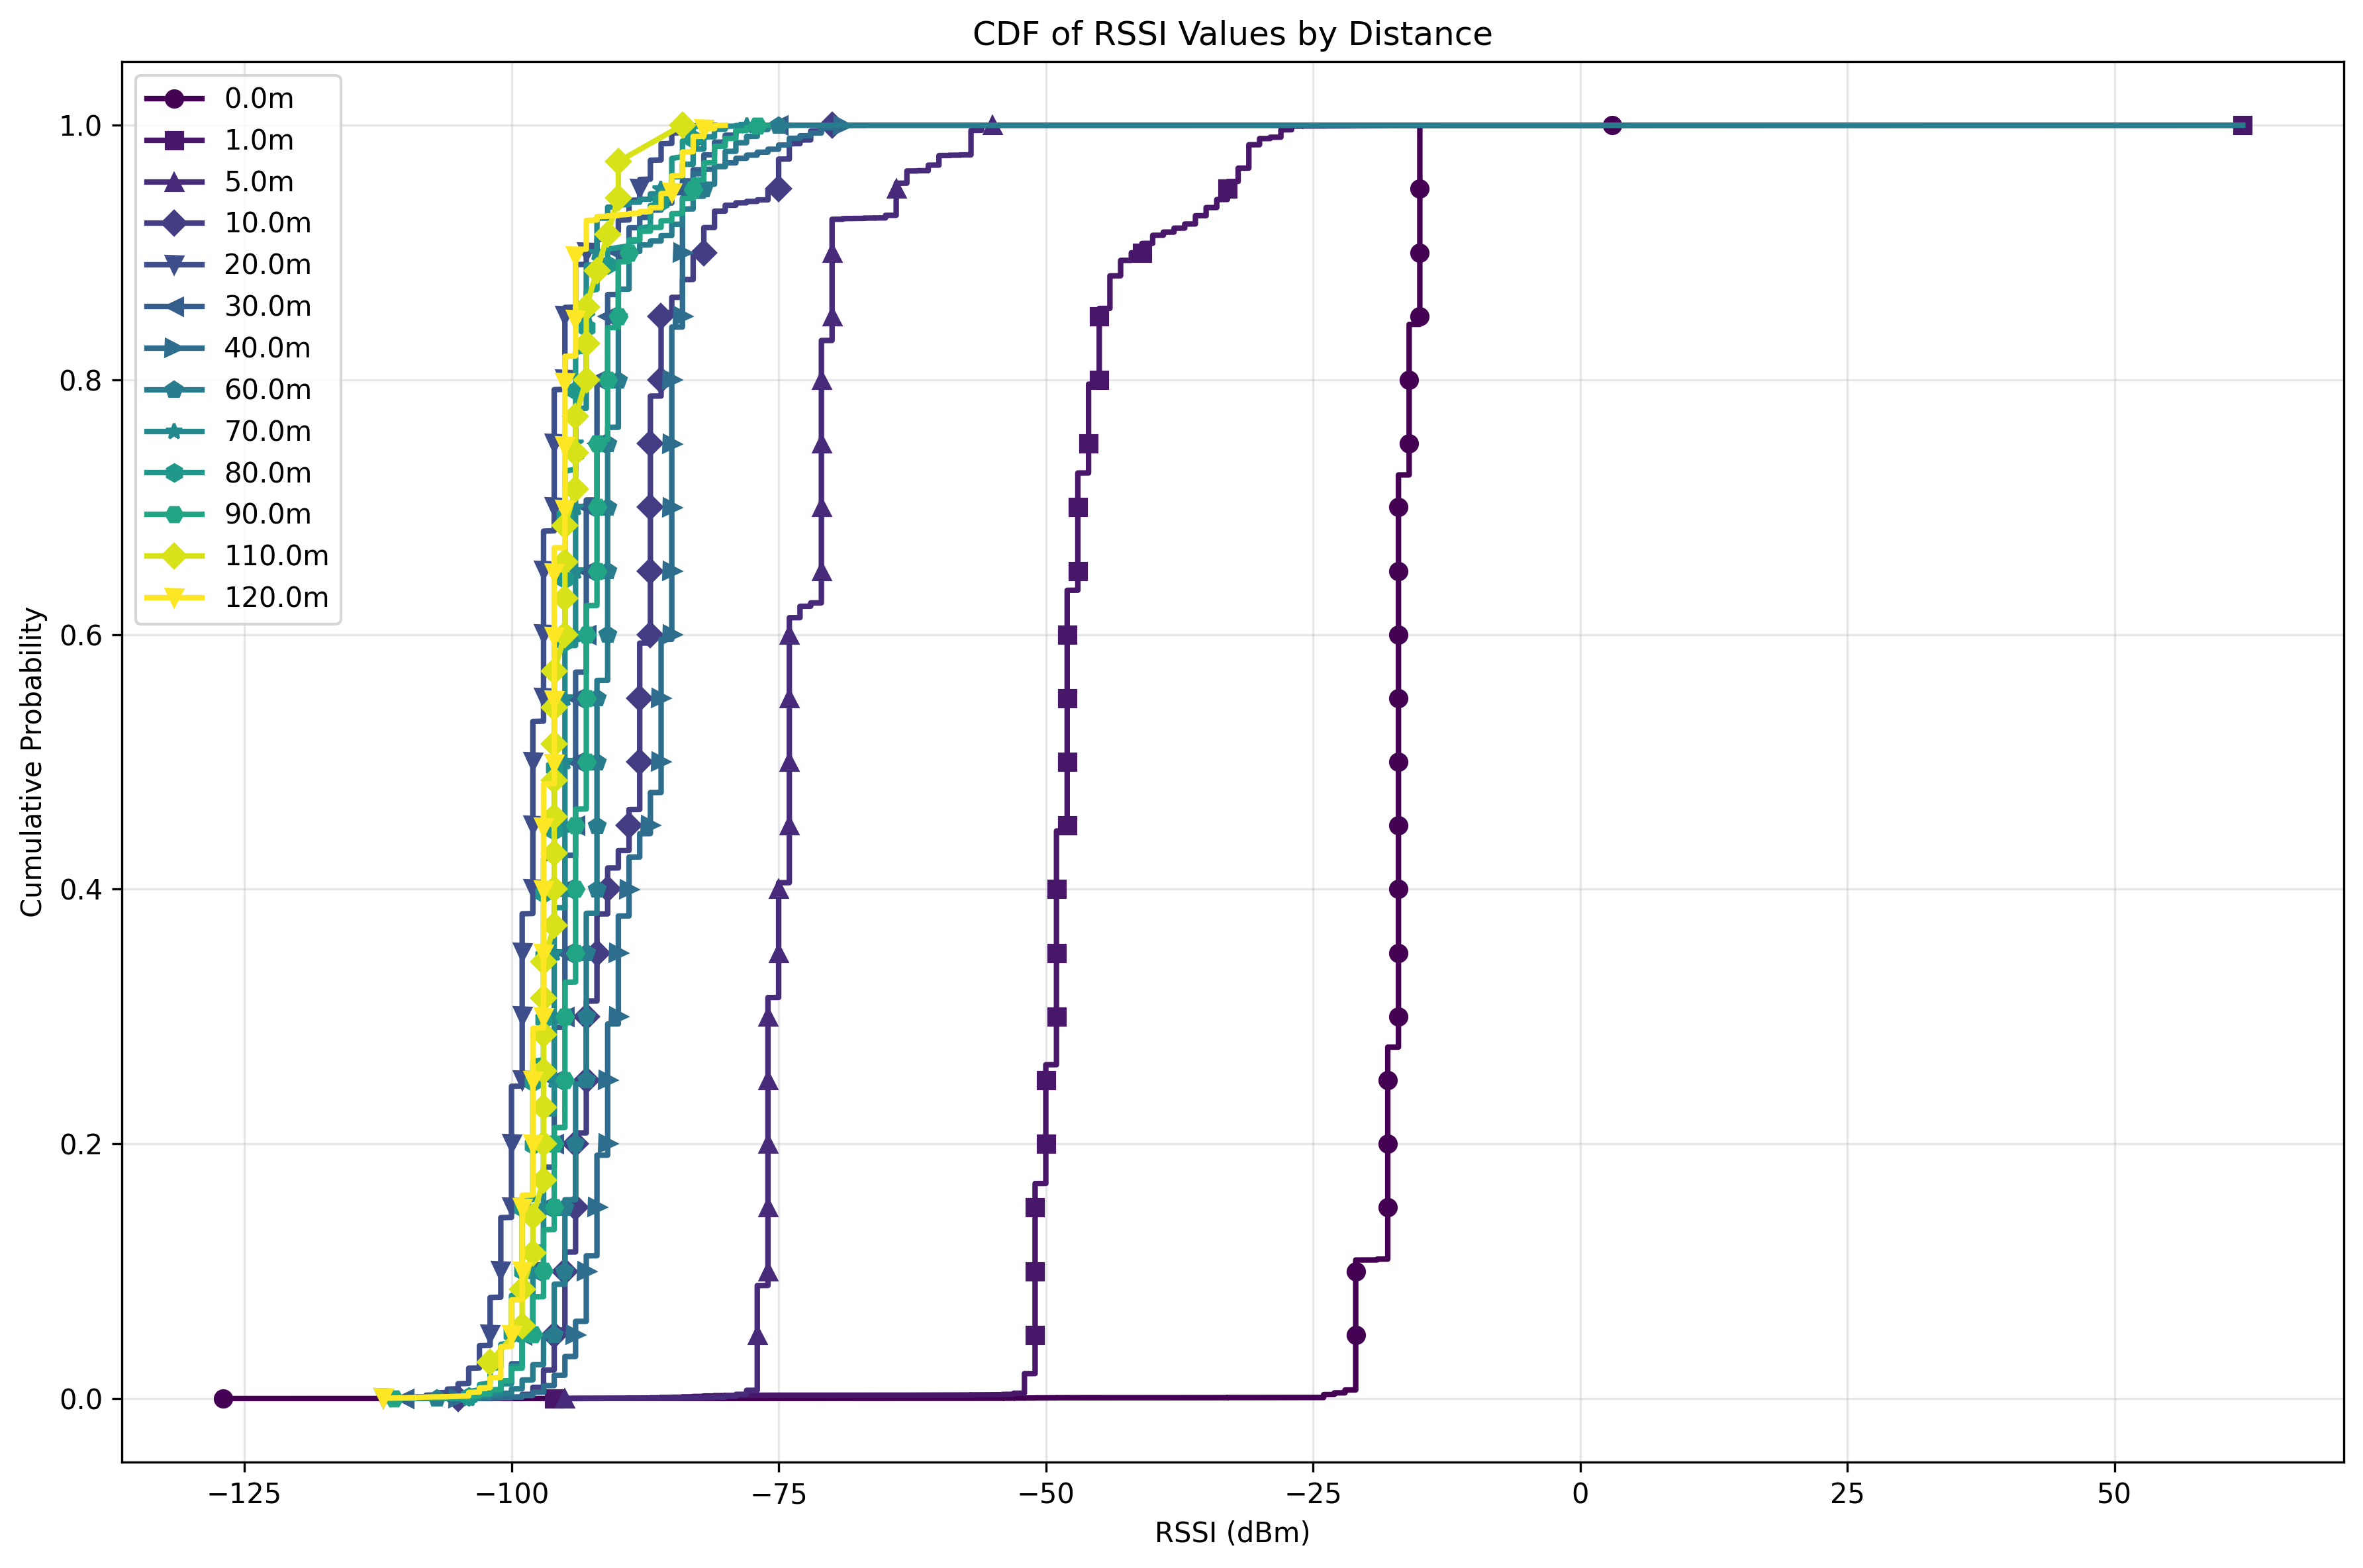
\includegraphics[width=0.5\textwidth]{figures/rssi_cdf.png}
     \caption{CDF of the RSSI vs. distance}
     \label{fig:rssi-cdf}
 \end{figure}

Figure \ref{fig:rssi-cdf} shows the CDF of the RSSI values at different distances. On the X axis we can see the RSSI values in dBm, and on the Y axis the cumulative distribution function (CDF) of the RSSI values recorded at that distance.

\begin{figure}[htbp]
     \centering
     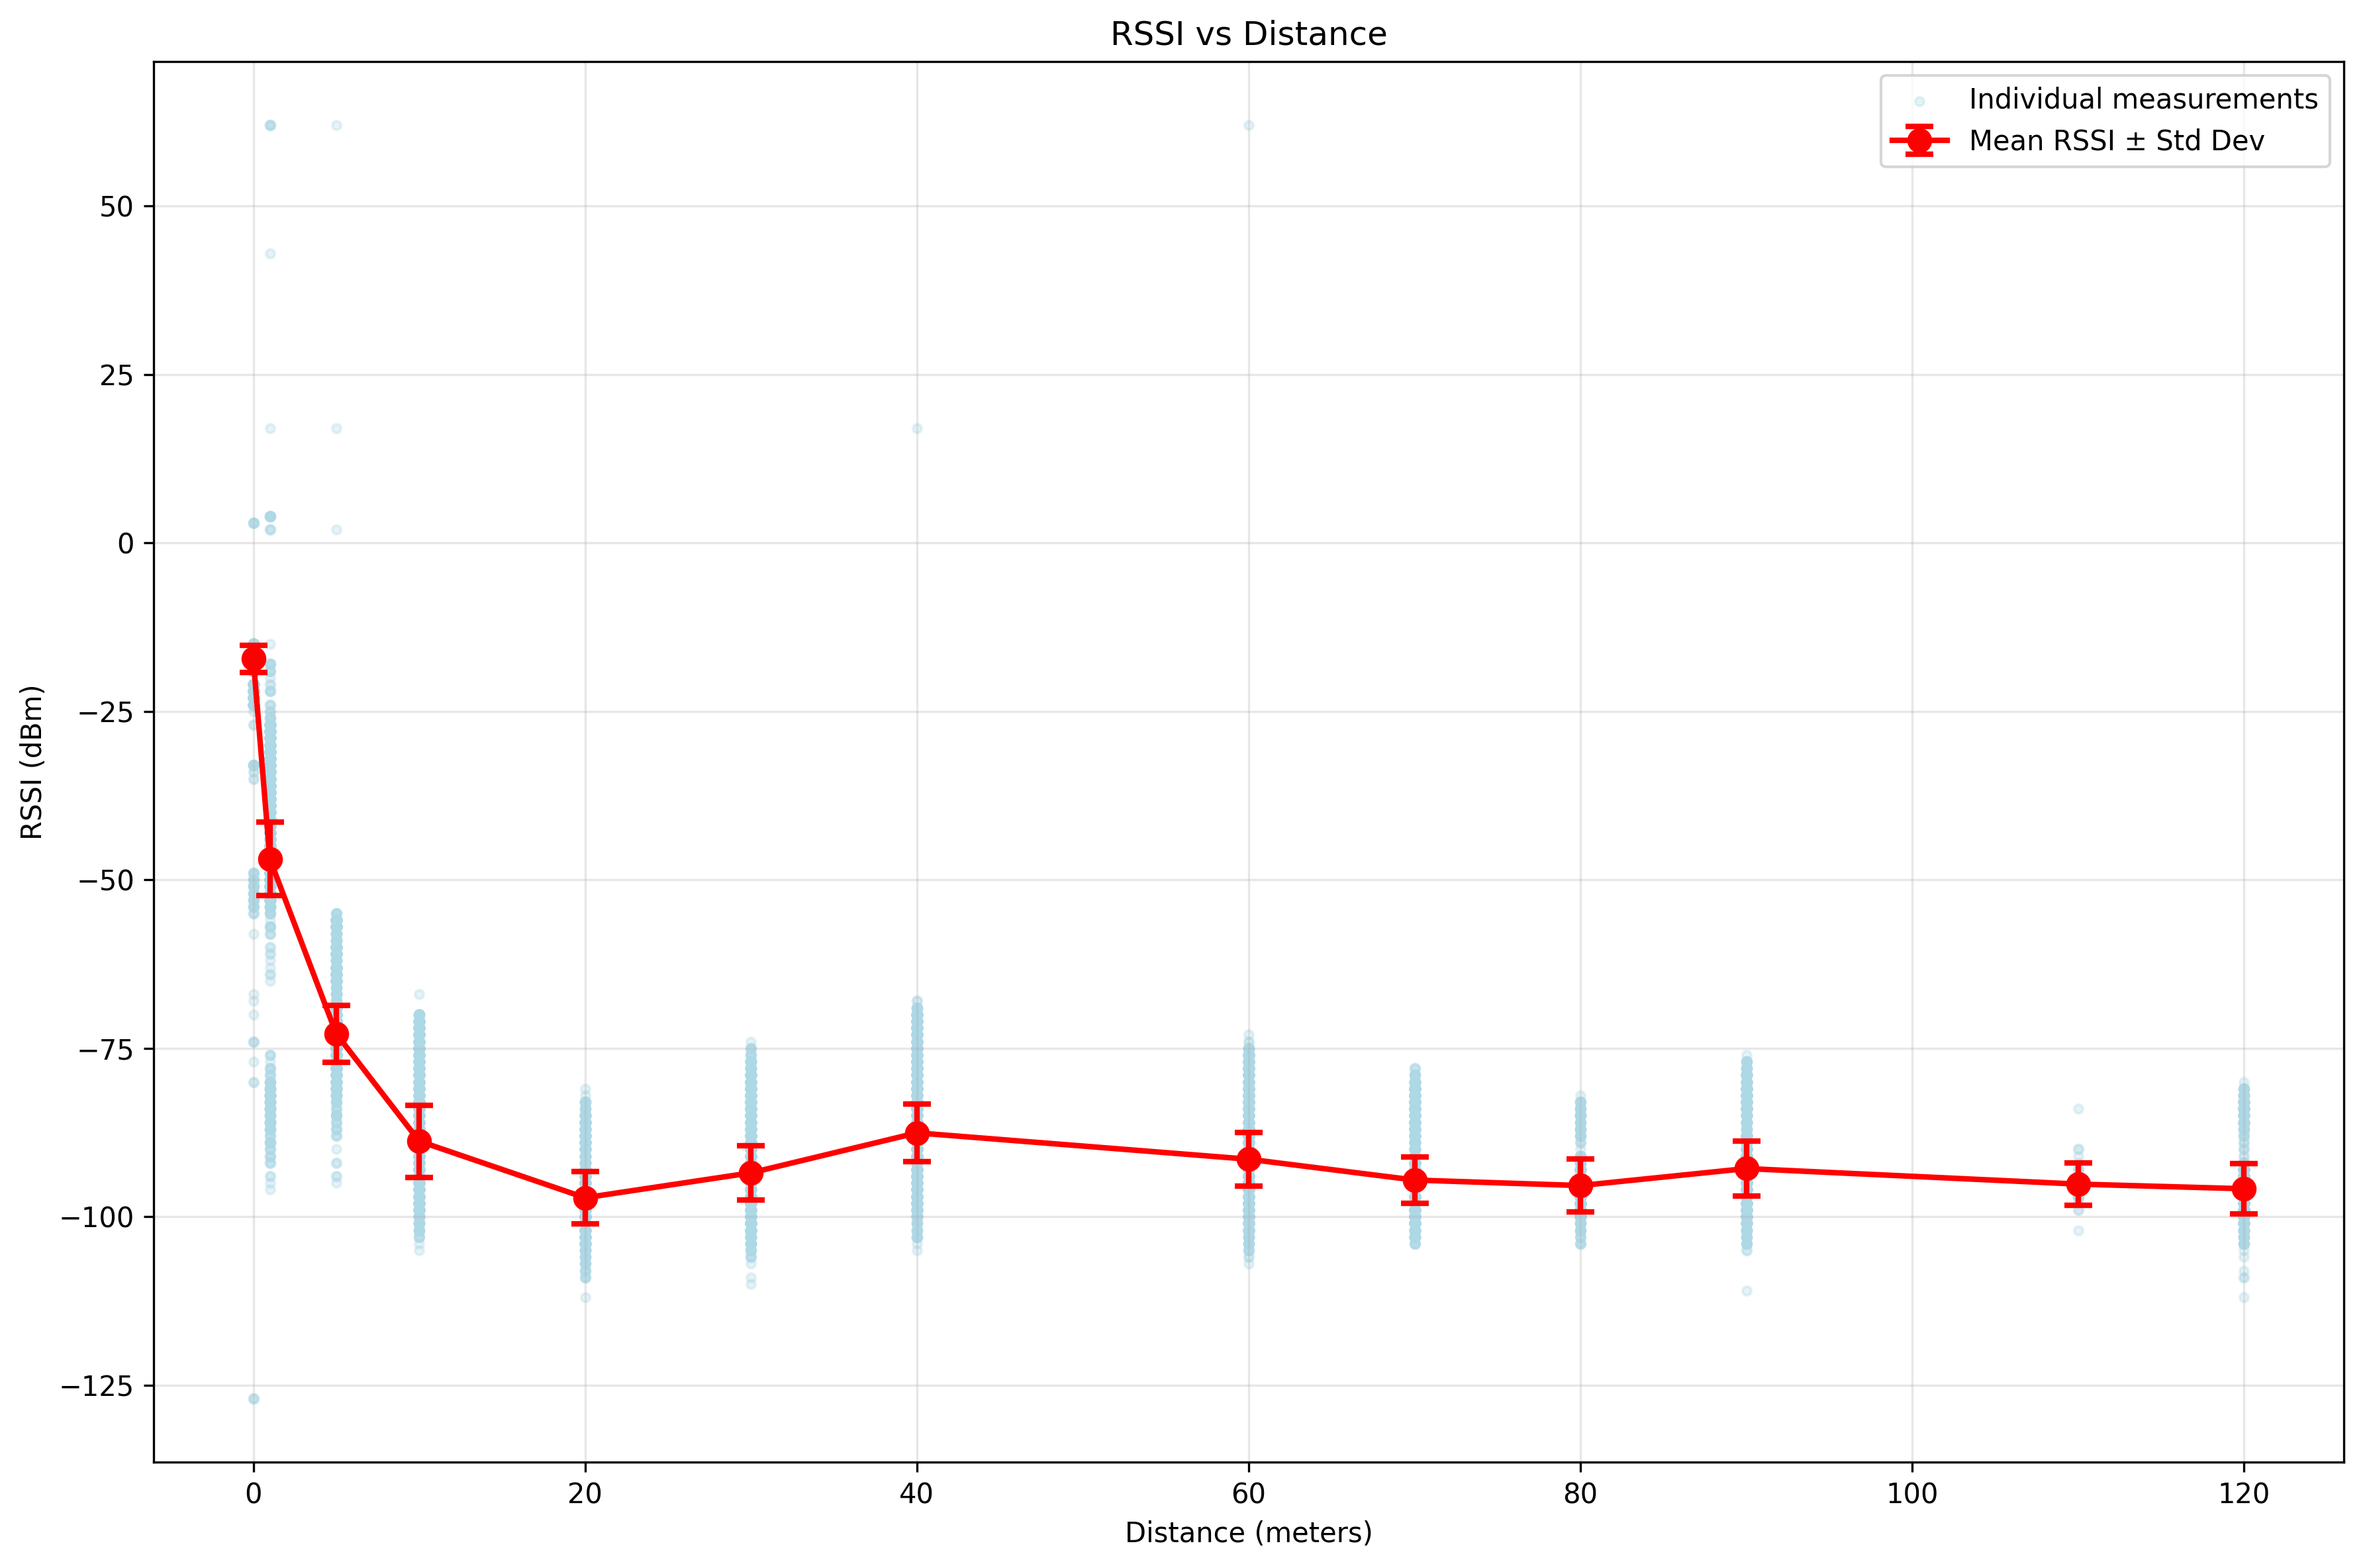
\includegraphics[width=0.5\textwidth]{figures/rssi_vs_distance.png}
     \caption{RSSI vs. distance}
     \label{fig:rssi-distance}
 \end{figure}

Figure \ref{fig:rssi-distance} shows how the RSSI changes with distance. Each point represents the mean RSSI value recorded at the distance specified, with the bars indicating standard deviation.
This plot clearly shows an expected power law decrease of the RSSI as the distance increases.

\subsection{Simulations}
After finishing the empirical testbed data collection experiment, we used the collected data to derive the signal parameters for the Bluetooth signal path loss model, that was used in the ONE simulator to simulate different experiment topologies.
We used an Red-Black tree to store the distance value as keys, with the RSSI values as values, and interpolated for distance points between the keys.

\begin{figure}[htbp]
     \centering
     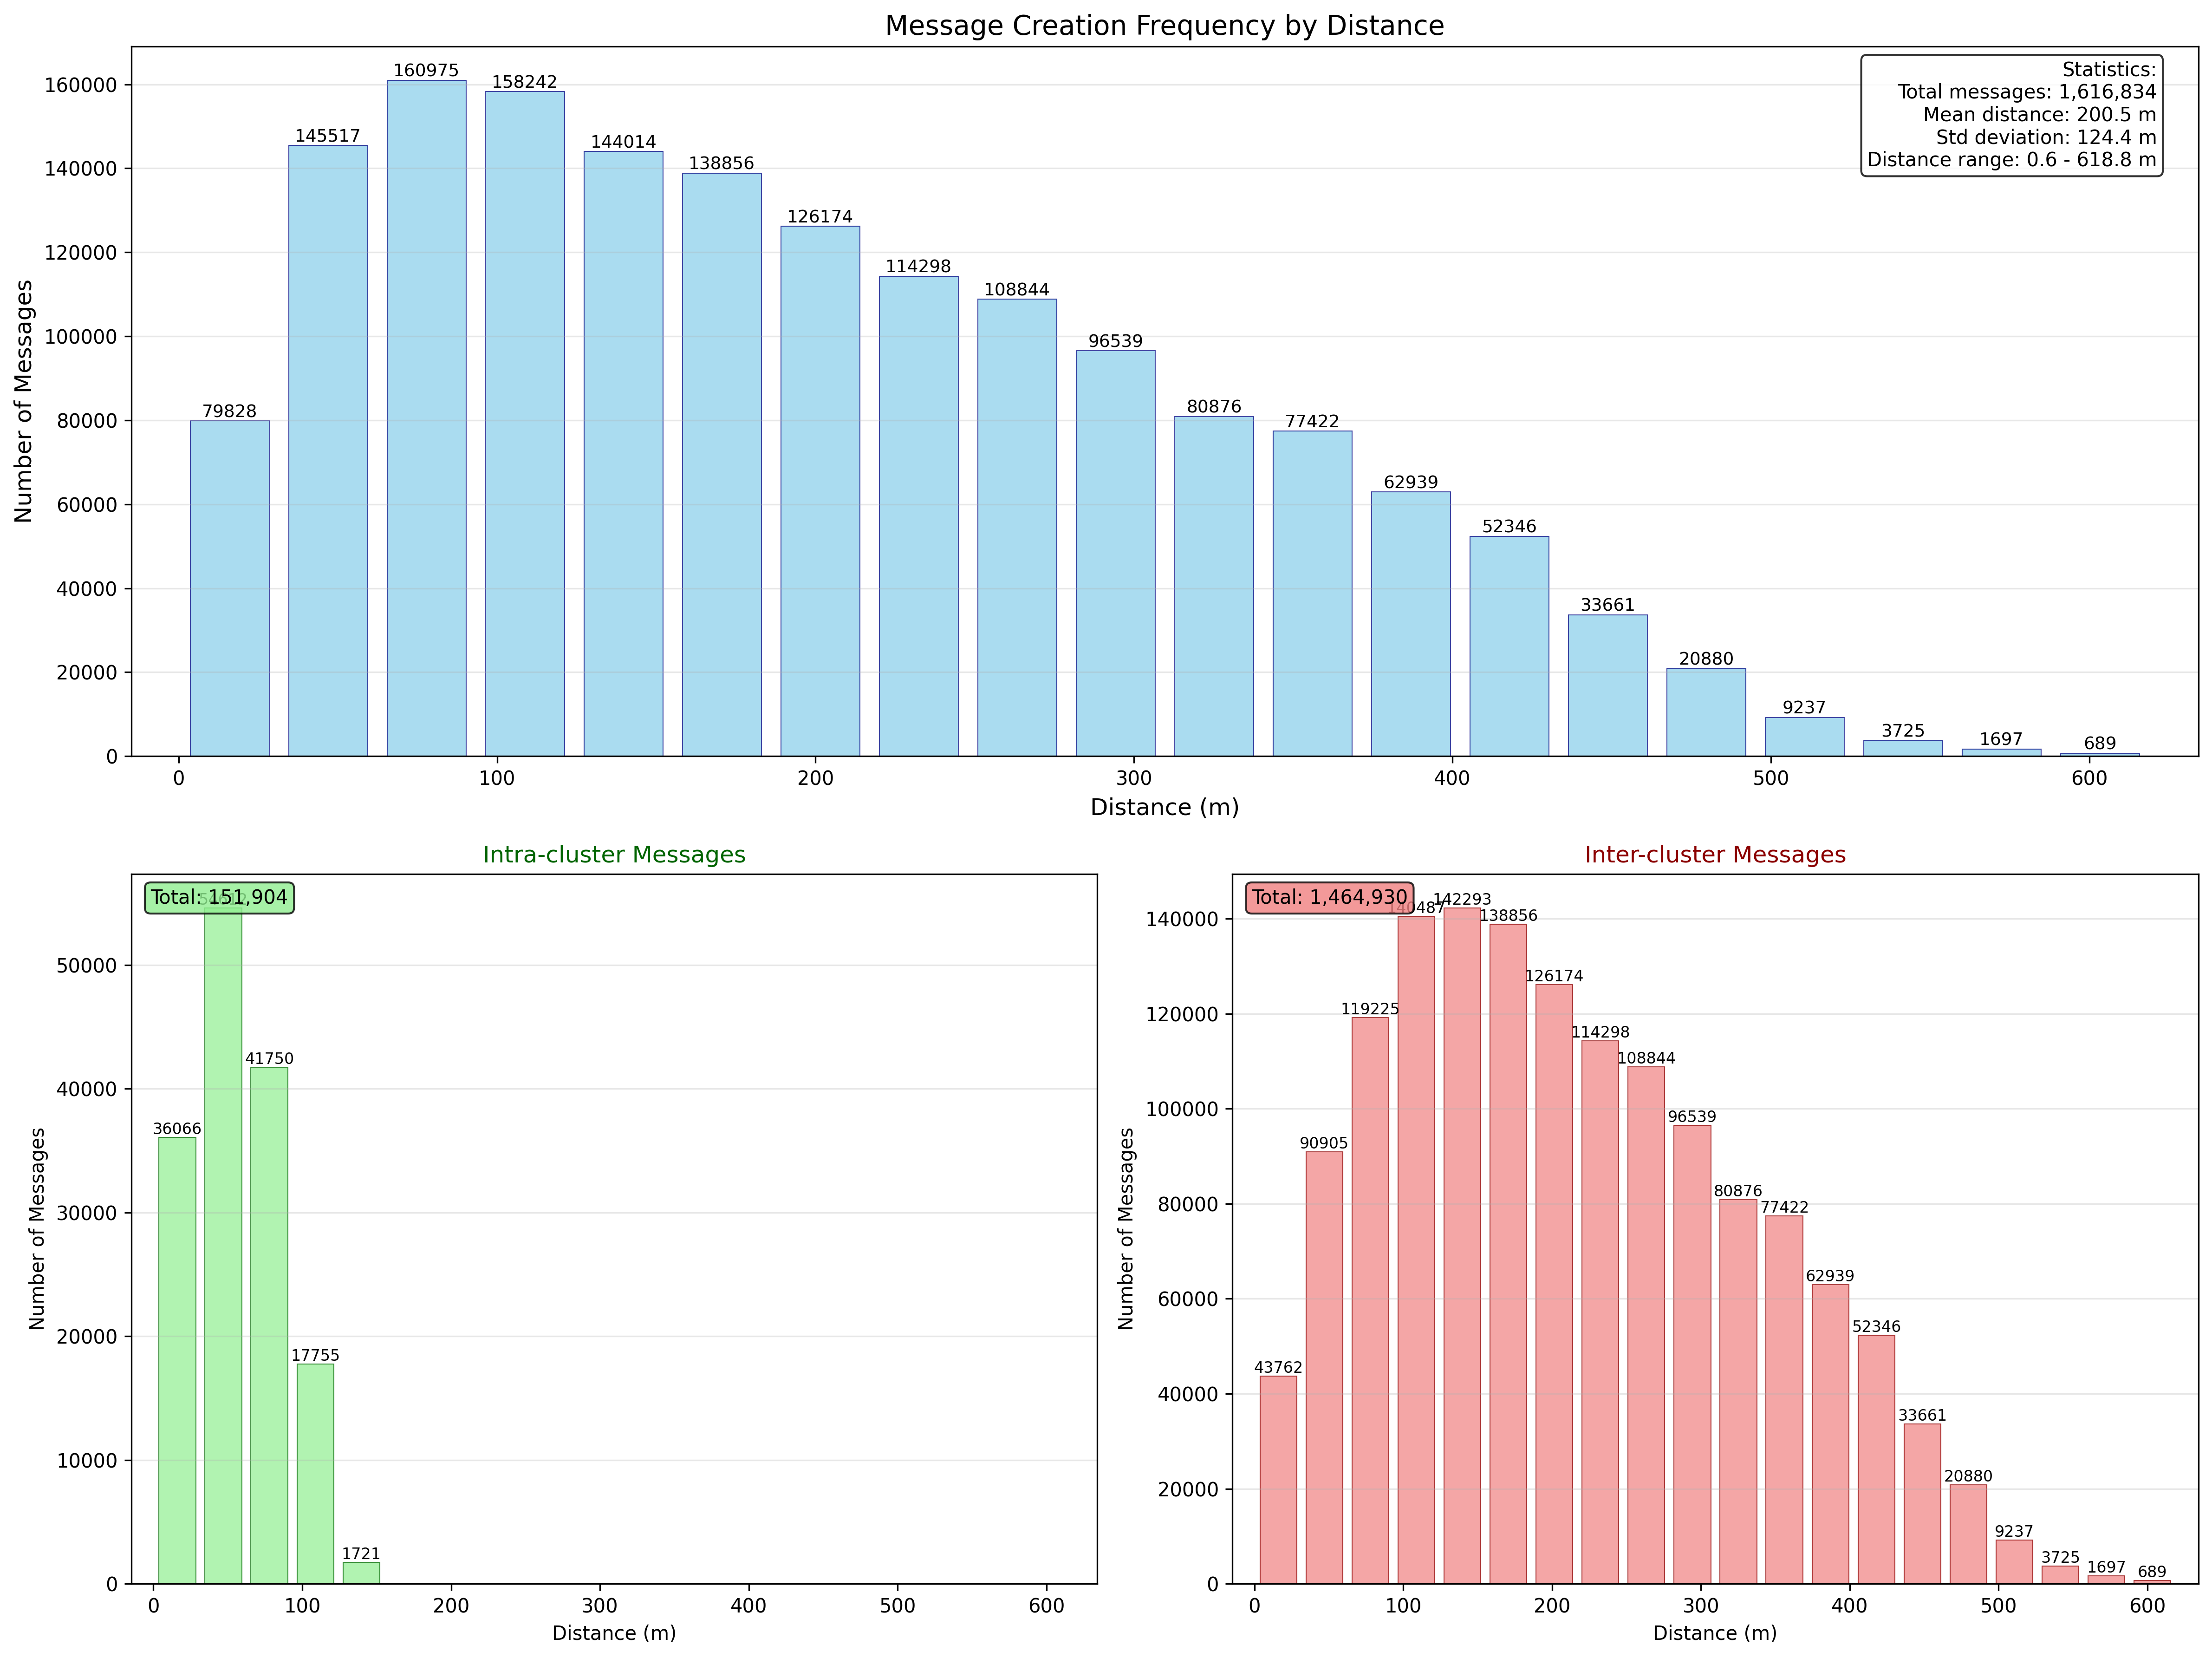
\includegraphics[width=0.5\textwidth]{figures/message-distance-distribution.png}
     \caption{Message distance distribution}
     \label{fig:message-distance}
 \end{figure}

Figure \ref{fig:message-distance} shows the distribution of the message distances that were generated. In every run, every host attempted to message every other host in the simulation, regardless of whether that host was directly reachable.

\begin{figure}[htbp]
    \centering
    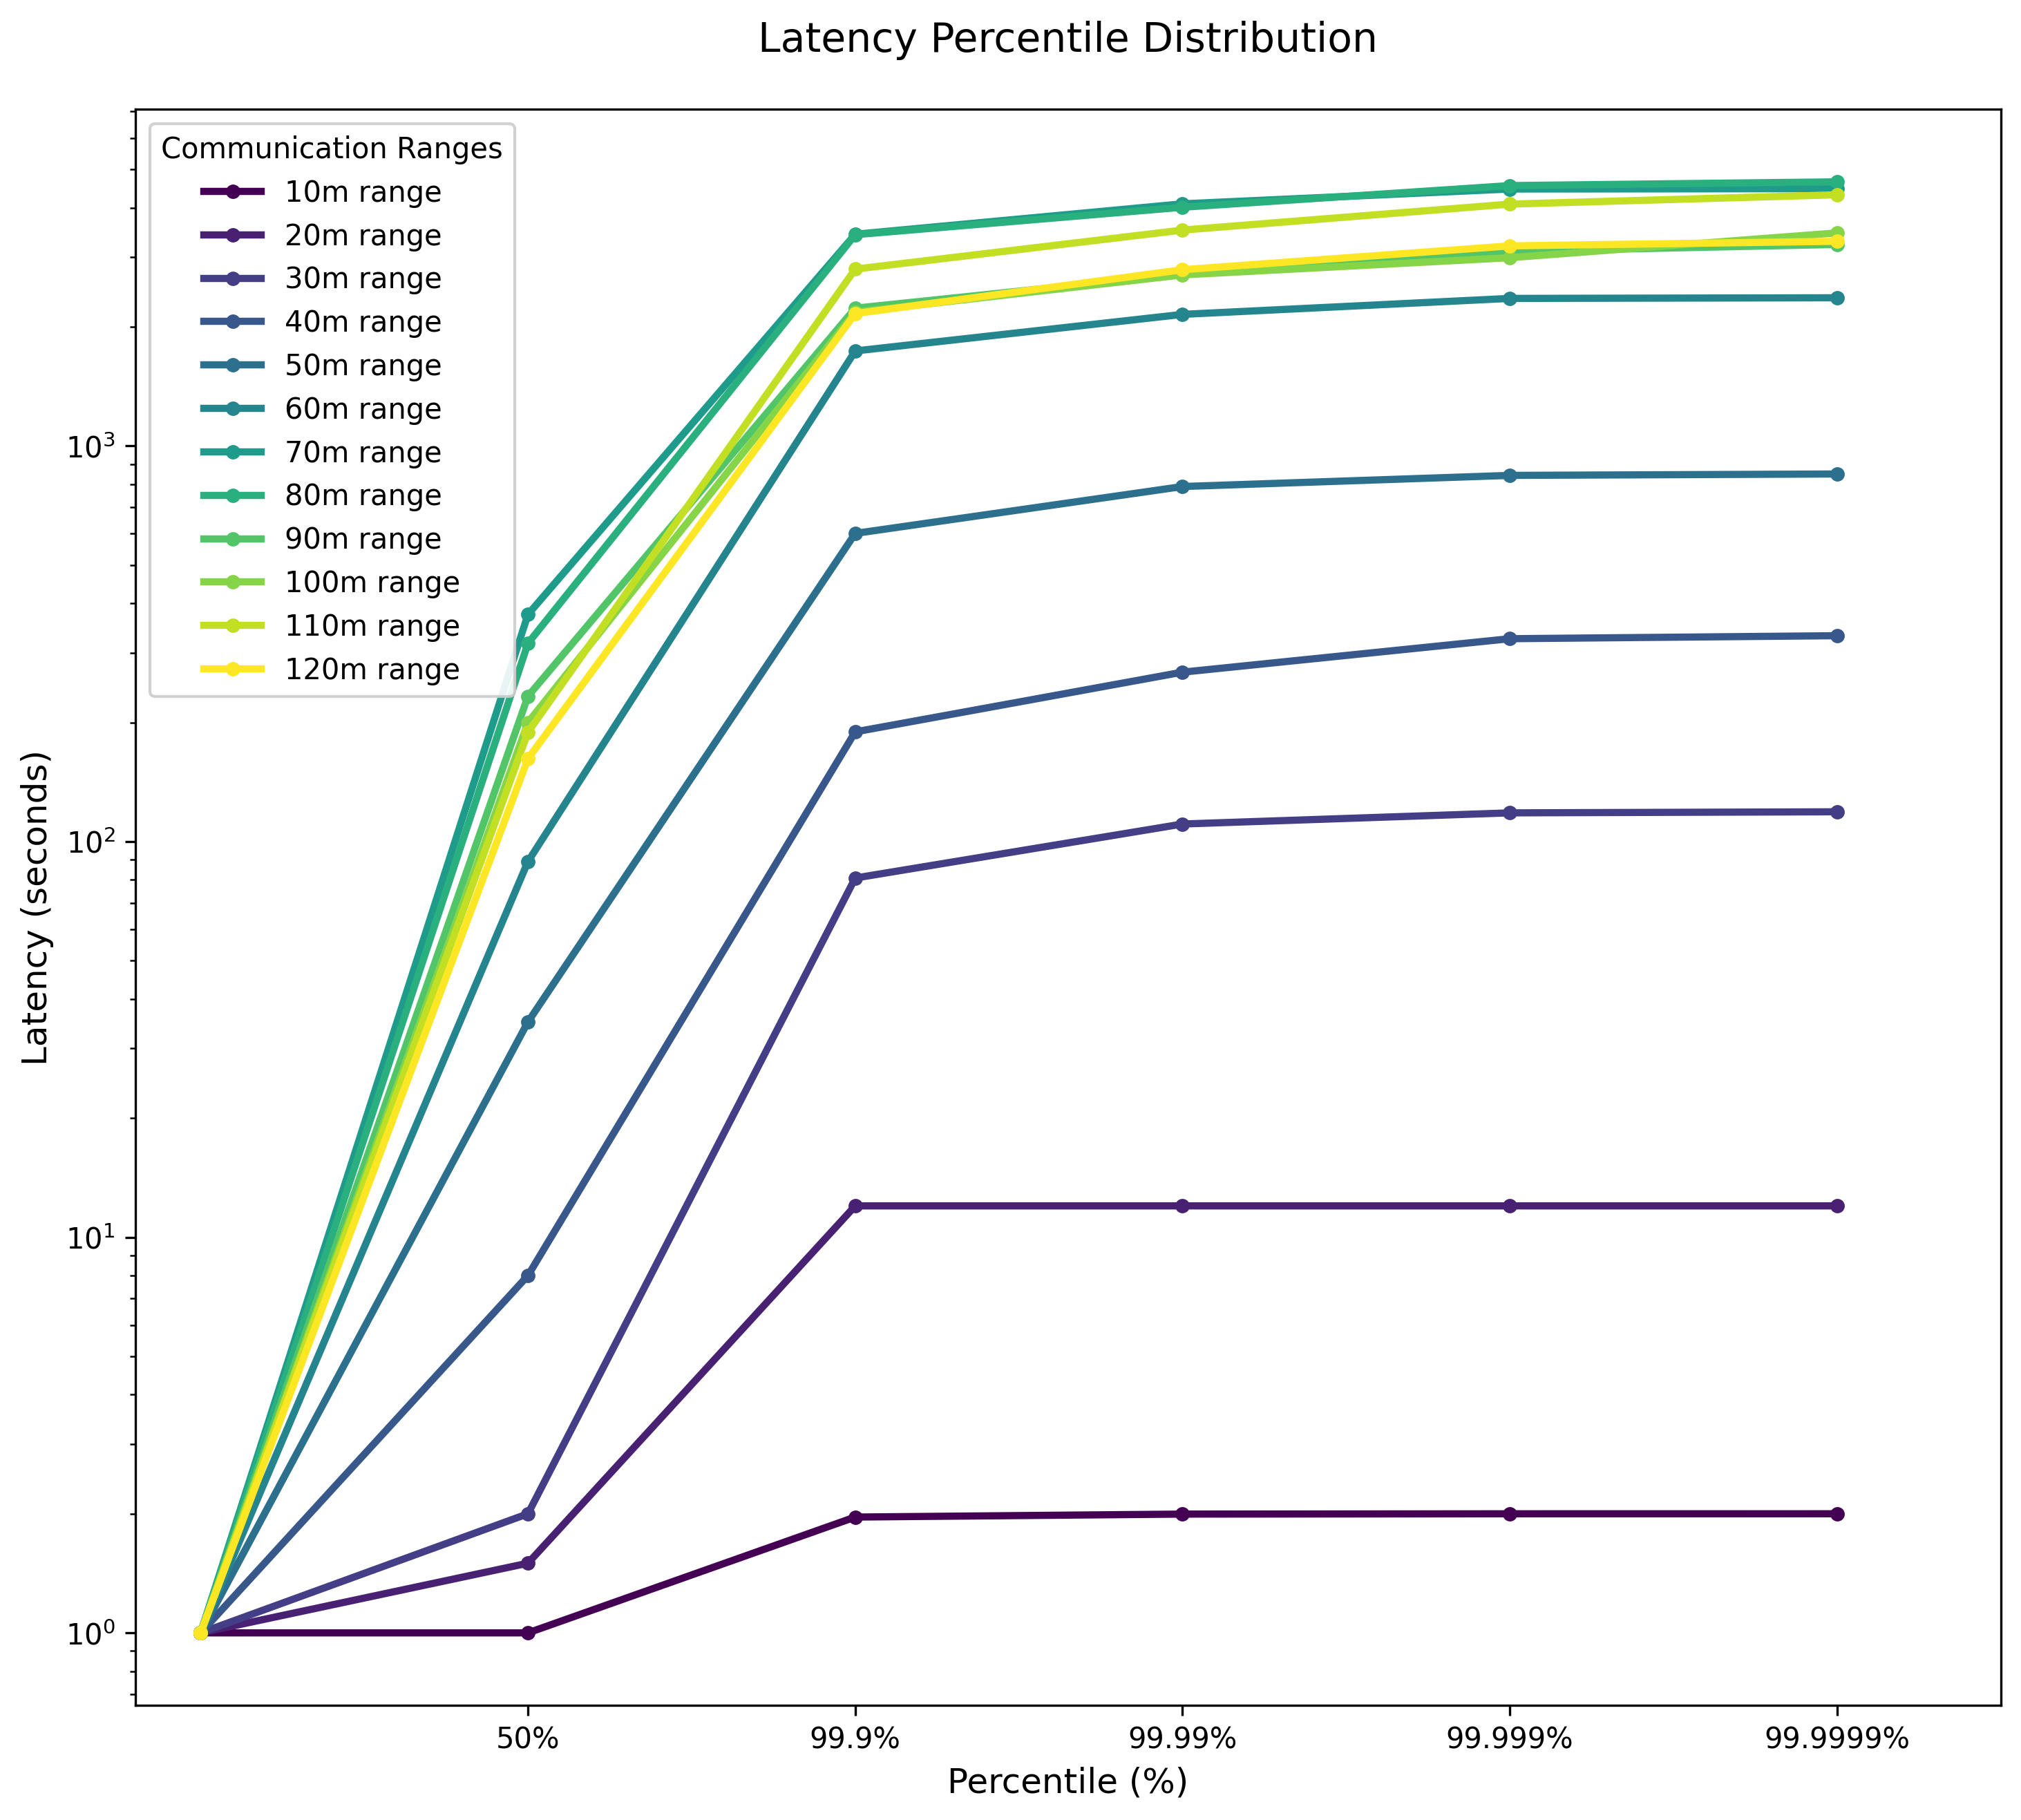
\includegraphics[width=0.5\textwidth]{figures/latency_percentiles.png}
    \caption{Latency percentiles}
    \label{fig:latency-percentiles}
\end{figure}

The figure \ref{fig:latency-percentiles} shows the latency measured in seconds, of delivering a message, as depending on the communication range.
The different communication radii are shown as distinct curves on the plot, and shows as expected a trend towards a lower latency with a lower communication radius. Lower communication radii in turn create less messages, which exhibit less strain on the message buffers of the individual hosts.

\begin{figure}[htbp]
     \centering
     \begin{minipage}[b]{0.47\textwidth}
         \centering
         \includegraphics[width=\textwidth]{figures/range120_maxdeg10_threshold10s.png}
     \end{minipage}
     \hfill
     \begin{minipage}[b]{0.47\textwidth}
         \centering
         \includegraphics[width=\textwidth]{figures/range120_maxdeg10_threshold240s.png}
     \end{minipage}
     \caption{Topology overview - 120m range}
     \label{fig:topology-overview-120}
 \end{figure}

The figure \ref{fig:topology-overview-120} shows two identical topologies, in which the communication range, or the communication radius of the network interface of every node, has a range of 120 meters. The difference between them is the time threshold used for the middle plot; in the first plot, the threshold of 10 seconds was used, and in the latter the threshold was set to 240 seconds.
The center plot, the delivery probability plot, measures the probability of a message being delivered within the time threshold, as a heatmap between every pair of nodes in the network.
The color indicates the delivery probability: the delivery probability within that threshold becomes lower the more red the color is, and is greener when the delivery probability improves. A delivery probability of 1.0 indicates all messages have been delivered within that threshold, and a delivery probability of 0.0 indicates that no message was delivered within the threshold.
The right matrix is the topological matrix: in this matrix, a connection between two nodes is indicated by the solid black color. Finally, the left matrix shows the distance between every two nodes: a more intense yellow indicates a higher distance, and a dark blue indicates less distance. It is easy to see that nodes within the same cluster are the closest to one another, and the clusters are the most visible in the intra-cluster topological matrix.
 \begin{figure}[htbp]
     \centering
     \begin{minipage}[b]{0.47\textwidth}
         \centering
         \includegraphics[width=\textwidth]{figures/range30_maxdeg10_threshold10s.png}
     \end{minipage}
     \hfill
     \begin{minipage}[b]{0.47\textwidth}
         \centering
         \includegraphics[width=\textwidth]{figures/range30_maxdeg10_threshold240s.png}
     \end{minipage}
     \caption{Topology overview - 30m range}
     \label{fig:topology-overview-30}
 \end{figure}

Similarly the figure \ref{fig:topology-overview-30} shows the same plots, but exhibits a different topology, as the host positions were randomized due to having a different communication range. As mentioned in previous chapters, the random number generator seed is determined by the communication radius and the message size, which was kept static.
In comparison, the 120m delivery probability plot at \ref{fig:topology-overview-120} exhibits a much higher delivery probability on average, as indicated by brighter green colors, in comparison to the 30m range.
These matrices were generated for every different topology and maximum node degree.

\clearpage
\begin{figure}[htbp]
     \centering
     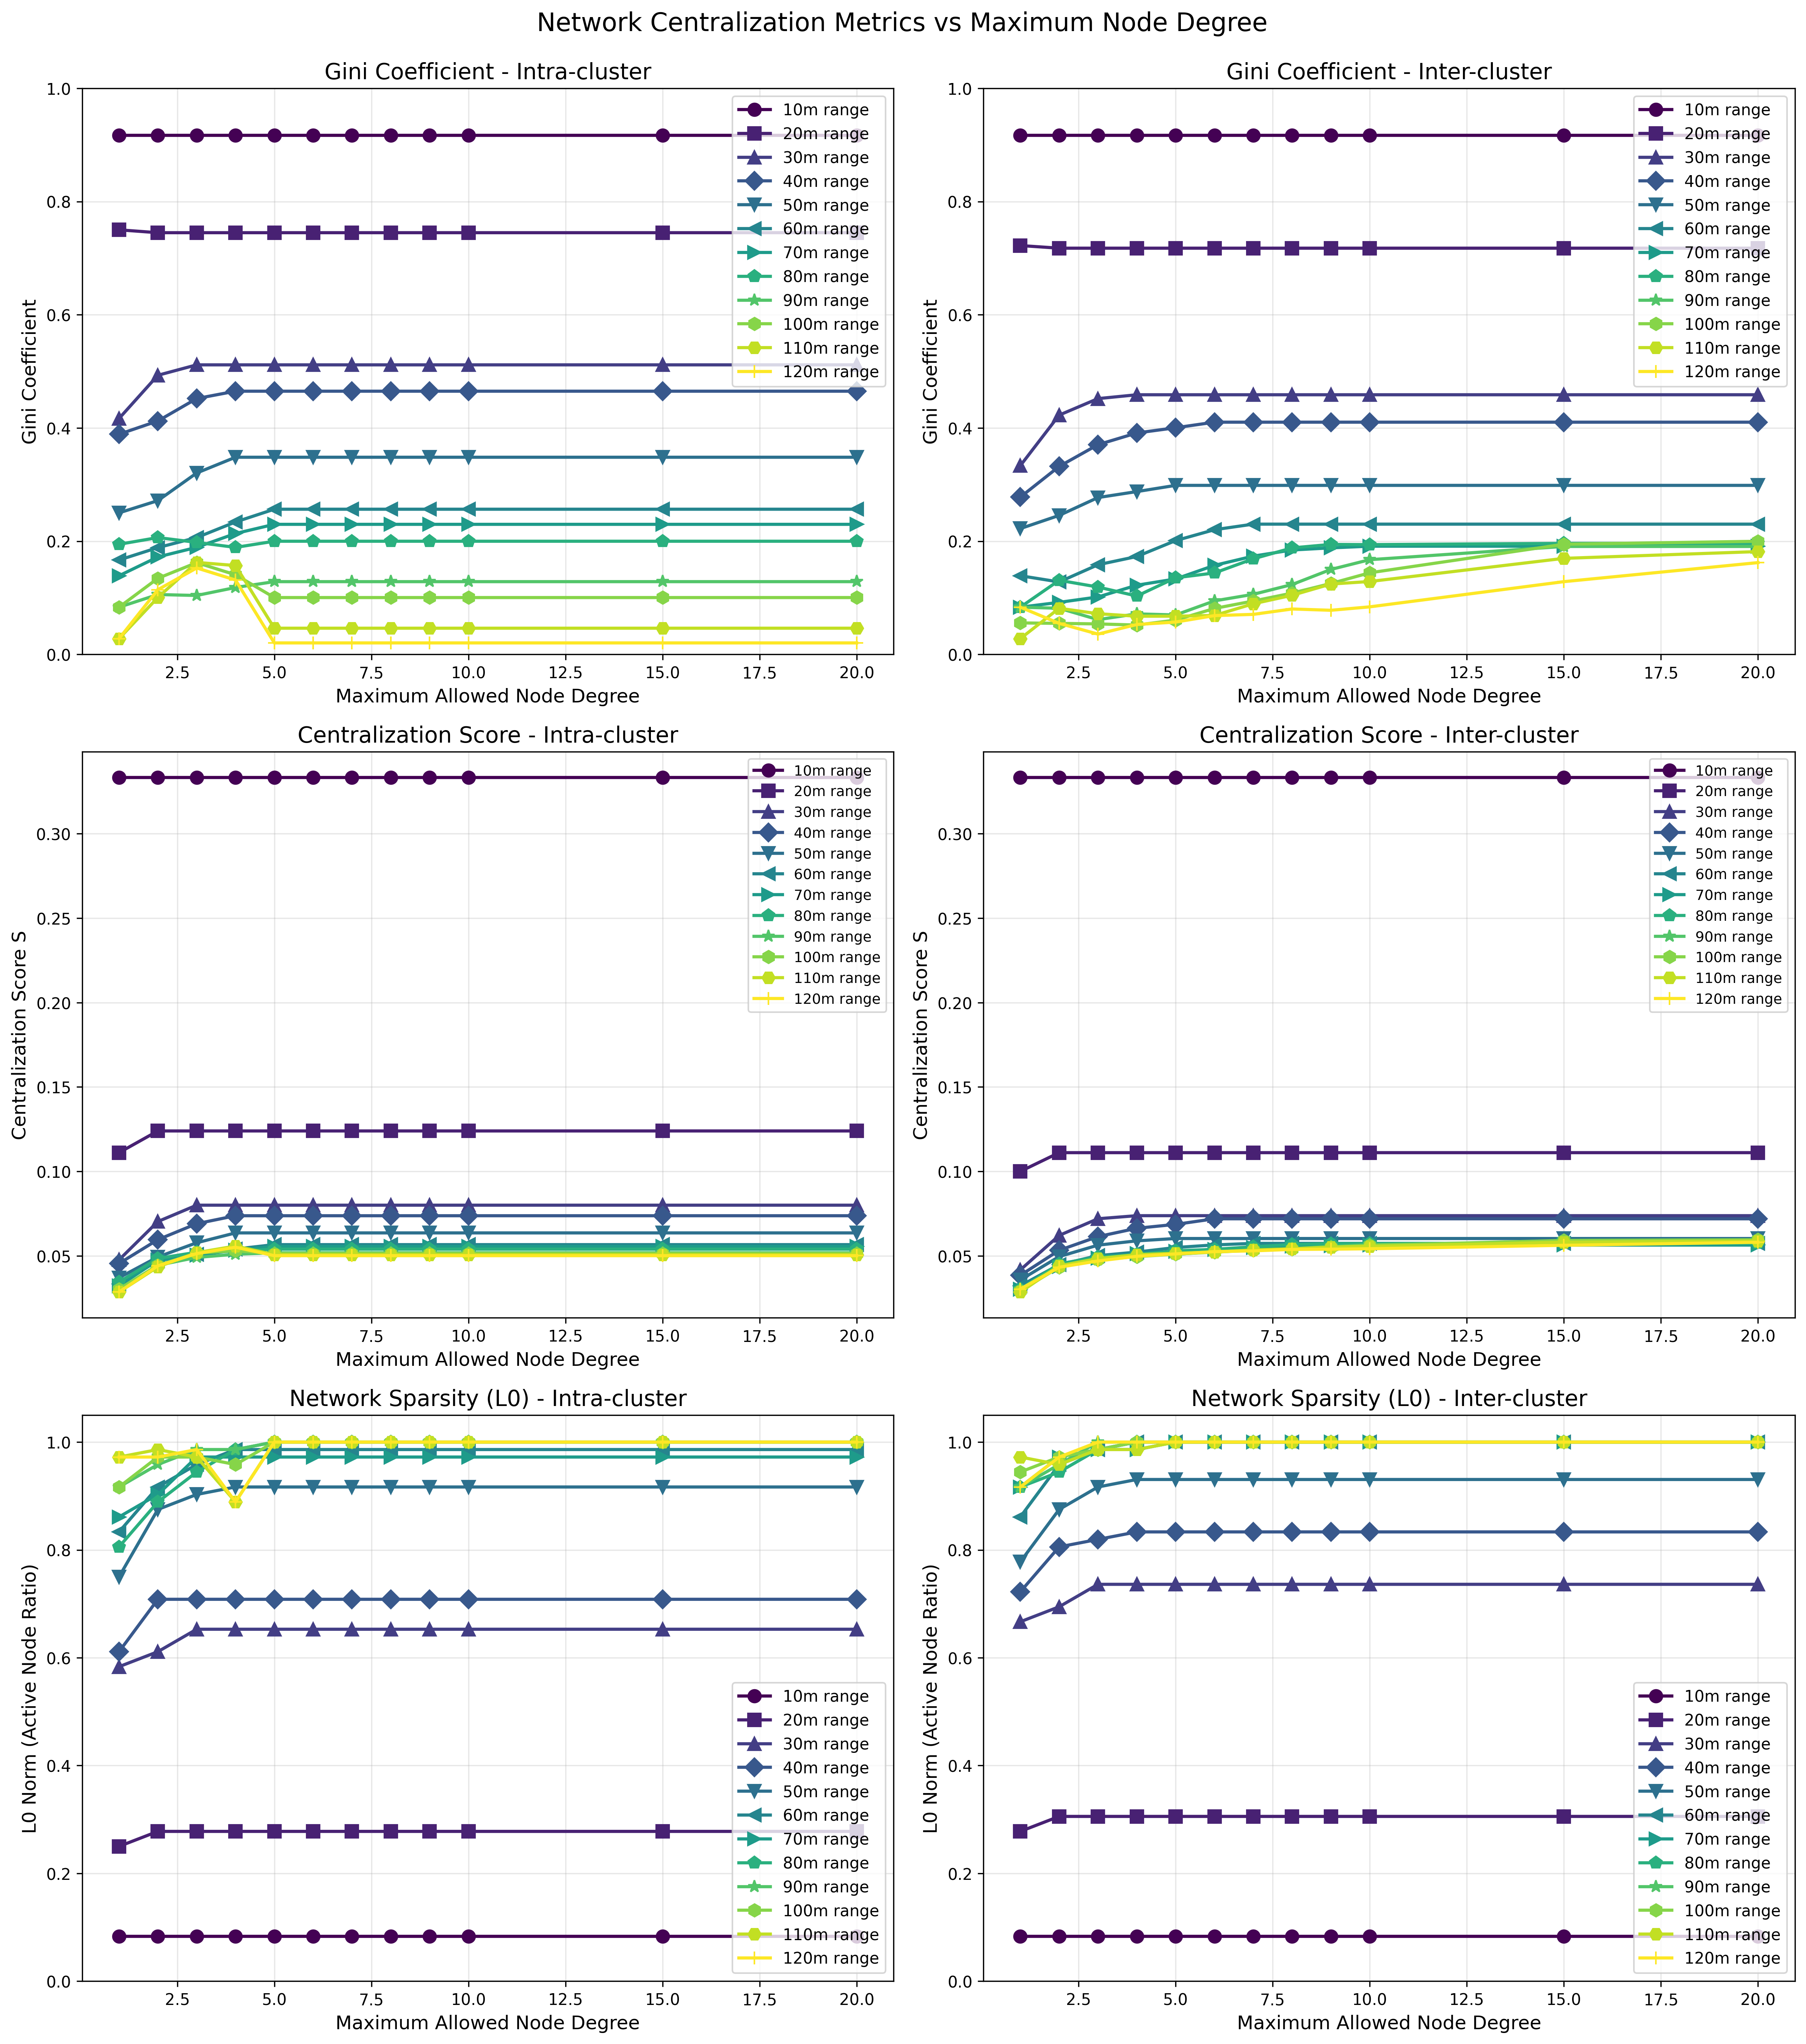
\includegraphics[width=0.85\textwidth]{figures/centralization_metrics_vs_max_degree.png}
     \caption{Centralization metrics vs. max degree}
    \label{fig:centralization-metrics}
 \end{figure}
\clearpage

Figure \ref{fig:centralization-metrics} shows how the maximum node degree, or the amount of parallel connections allowed per node, affects the different centralization metrics we measured, a subplot per communication mode.
In the intra-cluster mode, nodes were only allowed to communicate inside the same cluster, and messages were only created between nodes of the same cluster: there were no connections between nodes of different clusters, and no node attempted to message a node of a different cluster.
The inter-cluster mode causes a spike in the number of messages created, because nodes are allowed to communicate both with nodes of the same cluster, as well as outside their cluster: there is, insofar as the cluster membership is considered, no limitation on the communication: a node can communicate with all nodes in its communication radius.
The lack of communication limitation enables an exponential rise in the number of messages created: in the intra-cluster mode, 151,904 messages were created, as visible in \ref{fig:message-distance}. In the intra-cluster mode, where nodes can establish connections with all nodes within their range upto a maximum configured limit, the message generator generates a message for every pair in every possible permutation of the host list.
The same figure shows, that the inter-cluster mode featured over 1.4 million messages.
It is important to remark that there is still a limit on the maximum node degree, and each node's links do not churn: once a link has been established in a simulation, it persists until the end of the simulation.
At the top we can see the Gini coefficient vs. max node degree, at the middle the Centralization Score vs. max node degree, and at the bottom the L0 norm vs. max node degree, which measured the number of non-zero node degrees.